\chapter{Ballot design and voting}
\label{ch:ballot_design_and_voting}

\section{Ballot design}

A punchscan ballot consists of two pages stacked atop each other, as shown in
figure \ref{fig:punchscan_ballot}. It is uniquely identified by a numerical ID
printed on both pages. The top page contains the questions asked as well as all
possible answers. Each answer is mapped to a symbol --- in this case the
letters `a', `b' and `c'. The bottom page contains the same symbols, which can
be seen through cutouts in the top page when stacked atop each other. Both the
mapping of answers to symbols on the top page, as well as the order of symbols
on the bottom page, are independent random permutations per ballot. Multiple
questions can also be printed on the same ballot without loss of functionality
or privacy, as will be discussed later.

\begin{figure}[h]
\centering
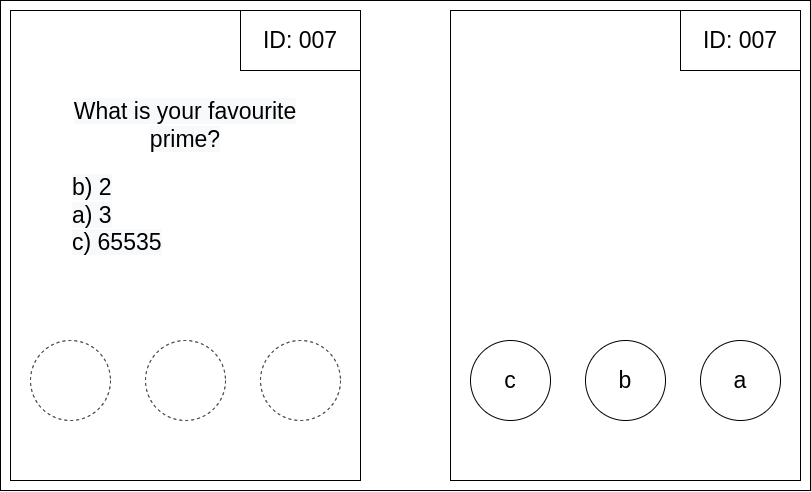
\includegraphics[width=0.7\textwidth]{../resources/high_level_ballot.drawio}
\caption{Punchscan ballot consisting of top (left) and bottom (right) page}
\label{fig:punchscan_ballot}
\end{figure}

\section{Voting process}

After having identified themselves at the polling place, a voter will have to
commit to getting to keep either the top or the bottom page of the ballot as a
receipt. They will then receive a random ballot, consisting of a top and bottom
page stuck together and enter the voting booth.

Within, the voter will read the question and decide on their answer. They will
look up which symbol their choice maps to on the top page, and then look
through which hole on the top page the corresponding symbol printed on the
bottom page is visible. They will then mark the corresponding slot using a
dauber --- a huge highlighter as used in Bingo --- thereby leaving a stain on
both the top as well as the bottom page of the ballot. The effect of having
marked their choice is shown in figure \ref{fig:punchscan_ballot_voted}.

The voter will then destroy the half of the ballot they will not keep by
feeding it through a shredder. They then exit the voting booth, and hand the
remaining half to a poll worker. The poll worker will scan the page, and feed
it through an OCR software. The voter gets to see and confirm that the scanned
page, including the detected choice, matches their physical copy. If so they
get to leave, keeping their scanned half of the ballot as a receipt.

\begin{figure}
\centering
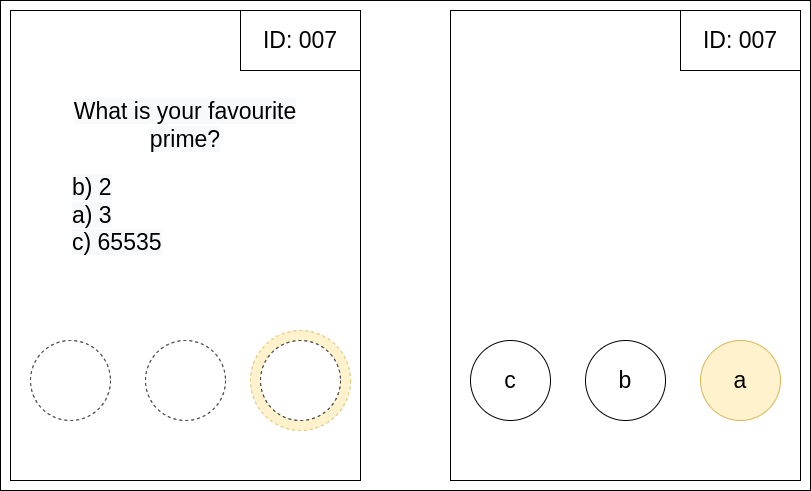
\includegraphics[width=0.7\textwidth]{../resources/high_level_ballot_voted_split.drawio}
\caption{Top (left) and bottom (right) pages of ballot after voter chose `3' as their favourite prime}
\label{fig:punchscan_ballot_voted}
\end{figure}
